%%%%%%%%%%%%%%%%%%%%%%%%%%%%%%%%%%%%%%%%%%%%%%%%%%%%%%%%%%%%%%%%%%%%%%
%% On jet mass corrections and transversity
%% May 10, 2013
%%%%%%%%%%%%%%%%%%%%%%%%%%%%%%%%%%%%%%%%%%%%%%%%%%%%%%%%%%%%%%%%%%%%%%
\documentclass[preprintnumbers,floatfix,nofootinbib]{revtex4}

\usepackage[tbtags]{amsmath}  % AMS math 
\usepackage{amssymb}          % AMS symbols
\usepackage{bm}               % bold math
\usepackage{graphicx}         % PostScript figures
\usepackage{hhline,multirow}  % for nicer tables
\usepackage{dcolumn}          % Align table columns on decimal point
\usepackage{slashed}

%%%%%% for draft
\newcommand{\todo}[1]{\marginpar{$\bullet$}\textbf{#1}}

%%%%%%  Definitions   %%%%%%%%%%%
  
\newcommand{\Pslash}{P \hspace{-0.24cm} / \,}
\newcommand{\kslash}{k \hspace{-0.21cm} / \,}
\newcommand{\lslash}{l \hspace{-0.19cm} / \,}
\newcommand{\nslash}{n \hspace{-0.24cm} / \,}
\newcommand{\vslash}{v \hspace{-0.21cm} / \,}
\newcommand{\Sslash}{S \hspace{-0.22cm} / \,}
\newcommand{\Dslash}{D \hspace{-0.22cm} / \,}
\newcommand{\epsslash}{\varepsilon \hspace{-0.18cm} / \,}
\newcommand{\Tr}{\operatorname*{Tr}\nolimits} % Trace operator
\newcommand{\xbj}{x}                   % Bjorken variable
\newcommand{\de}{d}                    % differential
\newcommand{\ii}{i}                    % imaginary unit

\allowdisplaybreaks[2]

\begin{document}

%%%%%%%%%%%%%%%%%%%%%%%%%%%%%%%%%%%%%%%%%%%%%%%%%%%%%%%%%%%%%%%%%%%%%%
%%%%%%%%%%%%%%%%%%%%%%%   TITLE    %%%%%%%%%%%%%%%%%%%%%%%%%%%%%%%%%%%
%%%%%%%%%%%%%%%%%%%%%%%%%%%%%%%%%%%%%%%%%%%%%%%%%%%%%%%%%%%%%%%%%%%%%%

\preprint{JLAB-THY-13-????}

\title{The role of jet mass corrections in polarized deep inelastic scattering}

\author{Alberto~Accardi$^{a}$, Alessandro~Bacchetta$^{b}$} 
\affiliation{
$^a$Jefferson Lab, Newport News, VA 23606, USA, and
Hampton University, Hampton, VA 23668, USA \\
$^b$Dipartimento di Fisica, Universit\`a degli Studi di Pavia, and INFN,
Sez. di Pavia, 27100 Pavia, Italy
}

\begin{abstract}

\end{abstract}

%\pacs{ }

%\keywords{ }

\maketitle


%%%%%%%%%%%%%%%%%%%%%%%%%%%%%%%%%%%%%%%%%%%%%%%%%%%%%%%%%%%%%%%%%%%%%%%%%
\section{Introduction}

%%%%%%%%%%%%%%%%%%%%%%%%%%%%%%%%%%%%%%%%%%%%%%%%%%%%%%%%%%%%%%%%%%%%%%%%%
\section{The Body}

We start from the case of semi-inclusive deep inelastic scattering integrated
over transverse momentum. The
general formula of the cross section is (see, e.g., \cite{Bacchetta:2008})
\begin{equation} 
\begin{split} 
\frac{d\sigma}{d\xbj \, dy\, d\psi \,dz}
&
=\frac{\alpha^2\, y}{8 z\, Q^4}\, 2 M W^{\mu \nu}\,
  L_{\mu \nu}
\\
&=
\frac{2 \alpha^2}{\xbj y\, Q^2}\,
\frac{y^2}{2\,(1-\varepsilon)}\, \biggl( 1+\frac{\gamma^2}{2\xbj} \biggr)\,
\biggl\{
F_{UU ,T} + \varepsilon\, F_{UU ,L}
+ S_\parallel \lambda_e\,
  \sqrt{1-\varepsilon^2}\; 
F_{LL}
%\nonumber 
\\  
&\quad
+ |\bm{S}_\perp|\,
\sqrt{2\,\varepsilon (1+\varepsilon)}\,
  \sin\phi_S\, 
F_{UT}^{\sin \phi_S }
+ |\bm{S}_\perp| \lambda_e\, \sqrt{2\,\varepsilon (1-\varepsilon)}\, 
  \cos\phi_S\, 
F_{LT}^{\cos \phi_S}
 \biggr\}.
\label{e:crossintsidis}
\end{split} 
\end{equation} 

Limiting ourselves
to the leading and first subleading term in the $1/Q$ expansion of the
cross section and to graphs with the hard scattering at tree level, we can
express the hadronic tensor as
\begin{equation} 
\begin{split} 
2M W^{\mu\nu} 
%&
&= 2z \sum_a   e_a^2 
\Tr \biggl\{
  \Phi^a (x) \gamma^\mu \Delta^a (z) \gamma^\nu
%\nonumber 
\\
& \quad 
- \frac{1}{Q\sqrt{2}} \biggl[
  \gamma^\alpha \nslash_+ \gamma^\nu \,
  \tilde{\Phi}^a_{A\, \alpha}(x)\, \gamma^\mu \Delta^a(z) 
+ \gamma^\alpha \nslash_- \gamma^\mu
  \tilde{\Delta}^a_{A\, \alpha} (z)\, \gamma^\nu 
  \Phi^a (x)  
  + \mathrm{h.c.} \,\biggr] \biggr\},
\label{eq1}
\end{split} 
\end{equation} 
with corrections of order $1/Q^2$, where the sum runs over the quark
and antiquark flavors $a$, and $e_a$ denotes the fractional charge of
the struck quark or antiquark. 

Instead of working with the fragmentation correlation function, $\Delta$, we
consider here the case where we insert a {\em jet correlation function}
\todo{AB: I don't know if we should include the gauge links explicitly}
\begin{equation} 
\Xi_{ij}(l) =\int
  \frac{\de^4\eta}{(2\pi)^4}\; e^{i k \cdot \eta}\,
    \langle 0|\, {\cal U}^{n_+}_{(+\infty,\eta)}
\,\psi_i(\eta)
             \bar{\psi}_j(0)\,
{\cal U}^{n_+}_{(0,+\infty)}\,   |0 \rangle
\label{e:xifull}
\end{equation} 
The correlator can be parametrized in terms of scalar functions, using 
the
vectors $l$ and $n_+$ 
\todo{AB: I don't know if we should include the last term or not. It has to do
with whether or not we want/need to address the complications related to the
gauge link}.
\begin{equation}
\begin{split} 
\Xi(l) = \Lambda A_1(l^2)\,{\bm 1} + A_2(l^2)\,\lslash 
+ \frac{\Lambda^2}{l \cdot n_{+}} \nslash_- \, B_{1}(l^2)
+ \frac{i \Lambda}{2 P \cdot n_{-}} [\lslash,\nslash_+ ] \, B_{2}(l^2)
\end{split} 
\end{equation} 

After the necessary integrations, we obtain a general form of the jet
correlation function in terms of jet components
\begin{equation} 
\Xi \equiv \int d l^+ d^2 l_T \, \Xi(l) 
\equiv \xi_1 \frac{\nslash_-}{2}+ 
\frac{\Lambda}{2 l^-}\,\xi_2 {\bm 1}
+\frac{\Lambda^2}{4 (l^-)^2}\,\xi_3 \nslash_+
+ i \frac{\Lambda}{2 l^-} \xi_4 
\frac{ \bigl[\nslash_-, \nslash_+ \bigr]}{2}.
\end{equation} 

To understand the nature of the $\xi$s, we consider the spectral
representation of the jet correlator
\begin{equation}
\Xi_{ij}(l) = \int \frac{d m_j^2}{2 \pi} J(m_j^2)\, \ii (\lslash +m_j) (-2 \pi \ii)
\delta(l^2 -m_j^2) \, \delta^2(l_T)
\label{e:spectral}
\end{equation} 
where the jet function $J$ has the property $\int dm_j^2 J(m_j^2) = 1$ and 
where the last $\delta$ comes from a choice of frame where the $l$ momentum
has no transverse components.
We obtain then
\begin{equation}
\begin{split} 
\int d l^+ d^2 l_T\, \Xi(l) &= \int \frac{d l^2}{2l^-} d^2l_T  
 \int \frac{d m_j^2}{2 \pi} J(m_j^2)\, \ii (\lslash +m_j) (-2 \pi \ii)
\delta(l^2 -m_j^2) \, \delta^2(l_T)
\\
& = \int d m_j^2 J(m_j^2) \Bigl( \frac{\gamma^+}{2} + \frac{m_j}{2 l^-} {\bm 1}
+\frac{m_j^2}{4 (l^-)^2} \gamma^- \Bigr)
\label{e:jetspectral}
\end{split} 
\end{equation} 
The result is in agreement with the general decomposition once we identify
\begin{align}
\xi_1 &= \int dm_j^2 J(m_j^2) = 1,
&
\xi_2 &= \int dm_j^2 \frac{m_j}{\Lambda} J(m_j^2) = \frac{\langle m_j \rangle}{\Lambda},
\\
\xi_4 &= 0,
&
\xi_4 &= \int dm_j^2 \frac{m_j^2}{\Lambda^2} J(m_j^2) = \frac{\langle m_j^2 \rangle}{\Lambda^2}.
\end{align} 


We need to consider also the quark-gluon correlator 
$\tilde{\Xi}_{D\, \alpha}$. Due to the absence of transverse-momentum effects,
the correlator corresponds to
\begin{equation}
{\Xi}_A^{\alpha}(l^-) = 
\Xi_D^{\alpha} (l^-)
%- \int d^2 l_T l_T^{\alpha}\,\Xi (l^-,l_T)
\label{e:DeltaA}
\end{equation}
where 
\begin{equation} 
\begin{split} 
\left(\Xi_D^{\mu} \right)_{ij} &=
\frac{1}{2}\, \sum_X
\int \frac{\de \eta^+\, \de^2 \bm{\eta}_T}{(2\pi)^{3}}\;
e^{\ii k \cdot \eta}\,
\langle 0|\,
{\cal U}^{n_+}_{(+\infty,\eta)}\,
i D^{\mu}(\eta)\,
\,\psi_i(\eta)|X\rangle
\langle X|
             \bar{\psi}_j(0)\,
{\cal U}^{n_+}_{(0,+\infty)}
|0\rangle \bigg|_{\eta^-=0} .
\label{e:DeltaD}
\end{split} 
\end{equation}  
with the covariant derivative being
 $\ii D^{\mu}(\eta) = \ii
\partial^{\mu}+ g A^{\mu}$.

By analogy with the standard fragmentation
correlator, we can decompose it in the following way
\begin{align}
\tilde{\Xi}_{A}^{\alpha}(l^-) = 
\frac{\Lambda}{4}\,\bigl(\tilde{\xi}_4 + \ii\,\tilde{\xi}_2\bigr)\, 
\ii \gamma_T^{\alpha} \nslash_-.
\end{align} 

Relations between correlation functions of different twist are provided
by the equation of motion for the quark field
\begin{equation}
  \label{e:quark-eom}
\bigl[ \ii \! \Dslash(\eta) - m_q \bigr] \psi(\eta)
 = \bigl[ \gamma^+ \ii D^-(\eta) + \gamma^- \ii D^+(\eta) 
       + \gamma_T^\alpha\, \ii D_\alpha(\eta) 
- m_q \bigr] \psi(\eta)
 = 0 ,
\end{equation}
where $m_q$ is the quark mass. Applying the equations of motion, we obtain the
following relations
\begin{align}
\tilde{\xi}_2 &=\xi_2 -  \frac{m_q}{\Lambda}\,\xi_1,
\\
\tilde{\xi}_4  &=\xi_4.
%- \int d^2 k_T \frac{k_T^2}{\Lambda^2}\, J^{\perp}.
\end{align} 
%\todo{AB: I've never introduced the last piece. Maybe we can simply skip the
%  second relation.}

The calculation of the hadronic tensor leads to the following result
\begin{equation} 
\begin{split} 
2MW^{\mu \nu} = 2 \sum_a e_a^2 \biggl[-g_\perp^{\mu\nu}\;f_1^a(\xbj)
+i\epsilon_\perp^{\mu\nu}\;g_1^a(\xbj)
\\
+i\frac{2M}{Q}\hat{t}^{[\mu}\epsilon^{\nu]\rho}_{\perp} S_{\perp \rho}
\Bigl(\xbj g_T (\xbj) + \frac{M_j -m_q}{M} h_1(\xbj \Bigr)
\biggr]
\label{wmunu}
\end{split} 
\end{equation} 

The cross section up to order $M/Q$ turns out to be
\begin{align}
F_{UU ,T} &= \xbj\,\sum_a e_a^2\,f_1^a(\xbj),
\\
F_{UU ,L} &= 0,
\\
F_{LL} &=\xbj\,\sum_a e_a^2\,g_1^a(\xbj),
\\
F_{UT}^{\sin \phi_S}&=0,
\label{e:FUTint}
\\
F_{LT}^{\cos \phi_S}&=-\xbj\,\sum_a e_a^2\, \frac{2M}{Q}\,
\biggl(\xbj  g_T^a(\xbj)
   + \frac{M_j -m_q}{M} \, h_{1}^a(\xbj) \biggr).
\end{align}


%%%%%%%%%%%%%%%%%%%%%%%%%%%%%%%%%%%%%%%%%%%%%%%%%%%%%%%%%%%%%%%%%%%%%%%%%
\section{Conclusions}


%%%%%%%%%%%%%%%%%%%%%%%%%%%%%%%%%%%%%%%%
%%%%%%%%% ACKNOWLEDGMENTS %%%%%%%%%%%%%%
%%%%%%%%%%%%%%%%%%%%%%%%%%%%%%%%%%%%%%%%

\begin{acknowledgments}
This work was supported by DOE contract No. DE-AC05-06OR23177,
under which Jefferson Science Associates, LLC operates Jefferson Lab, and 
by the Joint Research Activity ``Study of Strongly
Interacting Matter'' (acronym HadronPhysics3, Grant Agreement No. 283286) under
the 7th Framework Programme of the European Community.
\end{acknowledgments}

\appendix

%%%%%%%%%%%%%%%%%%%%%%%%%%%%%%
\section{Some details}

The calculation of the hadronic tensor can be done starting from the following
expression in TMD formalism
\begin{equation} 
\begin{split} 
2M W^{\mu\nu} 
%&
&= 2z \sum_a   e_a^2 \int d^2 \bm{p}_T d^2 \bm{k}_T 
\delta^2\Bigl(\bm{p}_T - \frac{\bm{P}_{h\perp}}{z}-\bm{k}_T\Bigr) 
\Tr \biggl\{
  \Phi^a (x,\bm{p}_T) \gamma^\mu \Delta^a (z,\bm{k}_T) \gamma^\nu
%\nonumber 
\\
& \quad 
- \frac{1}{Q\sqrt{2}} \biggl[
  \gamma^\alpha \nslash_+ \gamma^\nu \,
  \tilde{\Phi}^a_{A\, \alpha}(x,\bm{p}_T)\, \gamma^\mu \Delta^a(z,\bm{k}_T) 
+ \gamma^\alpha \nslash_- \gamma^\mu
  \tilde{\Delta}^a_{A\, \alpha} (z,\bm{k}_T)\, \gamma^\nu 
  \Phi^a (x,\bm{p}_T)  
  + \mathrm{h.c.} \,\biggr] \biggr\},
\label{eq2}
\end{split} 
\end{equation} 

The correlators $\Phi$ and $\Delta$ are usually written in terms of light cone
vectors $n_-$, $n_+$, which  are collinear to $P$ and $P_h$.
When including $1/Q$ corrections, we have to take into consideration the
difference between those vectors and the vectors $n'_-$ and
$n_+'$, which are collinear to $P$ and $q$. The difference is (see,
e.g., Eq.~(20) and (21) of \cite{Mulders:1995dh})
\begin{align}
n_+^{\mu} &= n_+^{\prime \mu}
%\frac{1}{\sqrt{2}} \Bigl[\hat{t}^{\mu} + \hat{z}^{\mu}\Bigr]
&
n_-^{\mu} &=  n_-^{\prime \mu}
%\frac{1}{\sqrt{2}} \Bigl[\hat{t}^{\mu} -\hat{z}^{\mu}
+ \frac{2 P_{h\perp}^{\mu}}{z Q \sqrt{2}}
%\Bigr]
.
\end{align} 

In the jet case under consideration here, we are integrating over 
$dz\, d^2\bm{P}_{h\perp}$  because we are not observing the kinematics of the
final state. 
Moreover, we have $k_T=0$ and $z=1$. 
The expression for the hadronic tensor becomes
\begin{equation} 
\begin{split} 
2M W^{\mu\nu} 
%&
&= 2 \sum_a   e_a^2 \int dz z \int d^2 \bm{P}_{h \perp} d^2 \bm{p}_T d^2
\bm{k}_T
\delta^2\Bigl(\bm{p}_T - \frac{\bm{P}_{h\perp}}{z}-\bm{k}_T\Bigr) 
\Tr \biggl\{
  \Phi^a (x,\bm{p}_T) \gamma^\mu \Xi^a \delta(z-1) \delta^2(\bm{k}_T) \gamma^\nu
%\nonumber 
\\
& \quad 
- \frac{1}{Q\sqrt{2}} \biggl[
  \gamma^\alpha \nslash_+ \gamma^\nu \,
  \tilde{\Phi}^a_{A\, \alpha}(x,\bm{p}_T)\, \gamma^\mu 
\Xi^a \delta(z-1) \delta^2(\bm{k}_T) 
+ \gamma^\alpha \nslash_- \gamma^\mu
  \tilde{\Xi}^a_{A\, \alpha} \delta(z-1) \delta^2(\bm{k}_T)\, \gamma^\nu 
  \Phi^a (x,\bm{p}_T)  
  + \mathrm{h.c.} \,\biggr] \biggr\}
\\
&= 2 \sum_a   e_a^2 \int d^2 \bm{p}_T 
\Tr \biggl\{
  \Phi^a (x,\bm{p}_T) \gamma^\mu \Xi^a  \gamma^\nu
%\nonumber 
\\
& \quad 
- \frac{1}{Q\sqrt{2}} \biggl[
  \gamma^\alpha \nslash_+ \gamma^\nu \,
  \tilde{\Phi}^a_{A\, \alpha}(x,\bm{p}_T)\, \gamma^\mu 
\Xi^a
+ \gamma^\alpha \nslash_- \gamma^\mu
  \tilde{\Xi}^a_{A\, \alpha} \, \gamma^\nu 
  \Phi^a (x,\bm{p}_T)  
  + \mathrm{h.c.} \,\biggr] \biggr\}.
\label{eq3}
\end{split} 
\end{equation} 
In the last line, we can neglect the component of vector $n_-$
perpendicular to $\hat{t}$ and $\hat{z}$, but we have to take it into account
in the preceding line:
\begin{equation} 
\begin{split} 
2M W^{\mu\nu} 
%&
&= 2 \sum_a   e_a^2  
\Tr \biggl\{\int d^2 \bm{p}_T \Bigl( 
  \Phi^a (x,\bm{p}_T) \gamma^\mu \Xi^a  \gamma^\nu \Bigr)
%\nonumber 
\\
& \quad 
- \frac{1}{Q\sqrt{2}} \biggl[
  \gamma^\alpha \nslash_+ \gamma^\nu \,
  \tilde{\Phi}^a_{A\, \alpha}(x)\, \gamma^\mu 
\Xi^a
+ \gamma^\alpha \nslash_- \gamma^\mu
  \tilde{\Xi}^a_{A\, \alpha} \, \gamma^\nu 
  \Phi^a (x)  
  + \mathrm{h.c.} \,\biggr] \biggr\}
\\
&= 2 \sum_a   e_a^2  
\Tr \biggl\{  \Phi^a (x) \gamma^\mu \Xi^a  \gamma^\nu
+  \frac{1}{Q\sqrt{2}}
\Phi_{\partial\,\alpha}^a (x) \gamma^\mu \Xi^{a} \Big\vert_{\slashed{n}_- \to 2 \gamma^{\alpha}} \gamma^\nu 
%\nonumber 
\\
& \quad 
- \frac{1}{Q\sqrt{2}} \biggl[
  \gamma^\alpha \nslash_+ \gamma^\nu \,
  \tilde{\Phi}^a_{A\, \alpha}(x)\, \gamma^\mu 
\Xi^a
+ \gamma^\alpha \nslash_- \gamma^\mu
  \tilde{\Xi}^a_{A\, \alpha} \, \gamma^\nu 
  \Phi^a (x)  
  + \mathrm{h.c.} \,\biggr] \biggr\}\biggr\vert_{\slashed{n}_- \to \slashed{n}_-'}.
\end{split}
\end{equation} 

The previous steps are pretty safe. The following are still to be checked. If
they are correct, the final result is simple and appealing:
\begin{equation}
\begin{split} 
2M W^{\mu\nu} 
%&
&= 2 \sum_a   e_a^2  
\Tr \biggl\{  \Phi^a (x) \gamma^\mu \Xi^a \gamma^\nu
-  \frac{1}{Q\sqrt{2}}
  \gamma^\alpha \nslash_+ \gamma^\nu \,
\Phi_{\partial\,\alpha}^a (x) \gamma^\mu \Xi^{a} 
%\nonumber 
\\
& \quad 
- \frac{1}{Q\sqrt{2}} \biggl[
  \gamma^\alpha \nslash_+ \gamma^\nu \,
  \tilde{\Phi}^a_{A\, \alpha}(x)\, \gamma^\mu 
\Xi^a
+ \gamma^\alpha \nslash_- \gamma^\mu
  \tilde{\Xi}^a_{A\, \alpha} \, \gamma^\nu 
  \Phi^a (x)  
  + \mathrm{h.c.} \,\biggr] \biggr\}\biggr\vert_{\slashed{n}_- \to \slashed{n}_-'}
\\
&= 2 \sum_a   e_a^2  
\Tr \biggl\{  \Phi^a (x) \gamma^\mu \Xi^a  \gamma^\nu
\\
& \quad 
- \frac{1}{Q\sqrt{2}} \biggl[
  \gamma^\alpha \nslash_+ \gamma^\nu \,
  \Phi^a_{D\, \alpha}(x)\, \gamma^\mu 
\Xi^a
+ \gamma^\alpha \nslash_- \gamma^\mu
  \Xi^a_{D\, \alpha} \, \gamma^\nu 
  \Phi^a (x)  
  + \mathrm{h.c.} \,\biggr] \biggr\}\biggr\vert_{\slashed{n}_- \to \slashed{n}_-'}
.
\label{eq4}
\end{split} 
\end{equation} 
where
\begin{equation}
 \Phi_{\partial}^{\alpha} (x) = \int d^2\bm{p}_T p_T^{\alpha} \Phi(x,\bm{p}_T)
= \frac{M}{2}\biggl\{ S_T^{\alpha} g_{1T}^{(1)}(x) \gamma_5
- S_L h_{1L}^{\perp (1)} \gamma^{\alpha} 
+ f_{1T}^{\perp (1)} \epsilon_T^{\beta \alpha} S_{T \beta}
- i h_{1}^{\perp (1)}\gamma^{\alpha}\biggr\}\nslash_+ 
\end{equation} 

%%%%%%%%%%%%%%%%%%%%%%%%%%%%%%%%%%%%%%%%%%%%%%%%%%%
\section{Explicit calculations of jet propagator}

To check some of the general statements about the jet propagator, we can
compute it at first oder in the coupling constant of some theory. 
Let us start
from a pseudoscalar Yukawa interaction. The corresponding Feynman diagram is
shown in Fig.~\ref{fig:selfen} on the left. 
The formula is
\begin{equation}
\begin{split} 
\Xi(l) &= \frac{i (\slashed{l} +m)}{l^2 - m^2}
\biggl(\int \frac{d^4 p}{(2 \pi)^4} i g \gamma_5
 (\slashed{l}-\slashed{p} +m) i g \gamma_5 
(2 \pi ) \delta \bigl[p^2 - m_{\pi}^2\bigr]
(2 \pi) \delta\bigl[(l-p)^2 - m^2\bigr] \biggr)
\frac{(-i) (\slashed{l} +m)}{l^2 - m^2}
\\
&\equiv
\frac{i (\slashed{l} +m)}{l^2 - m^2}
(A \slashed{l} + B m) 
\frac{(-i) (\slashed{l} +m)}{l^2 - m^2}
=
\frac{1}{\bigl(l^2 - m^2\bigr)^2}
\Bigl[\Bigl(m^2 (A-2B) +  A\, l^2 \Bigr) \slashed{l} 
+
\Bigl(l^2 (B-2A) +  B\, m^2 \Bigr) m \Bigr] 
\end{split} 
\end{equation} 
The first step is justified by the fact that we have only one external 
vector $l$, therefore in general the result of the calculation of the integral
in the first line can be writte in terms of
$\slashed{l}$ and $m$. 
Already at this level, it is possible to say that the function 
multiplying $\slashed{l}$ is different from that multiplying $m$. 

\begin{figure*}
  \centering
  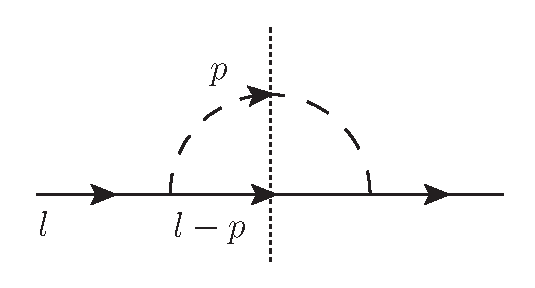
\includegraphics[width=0.3\linewidth]{selfen_cut}
  \hfil
  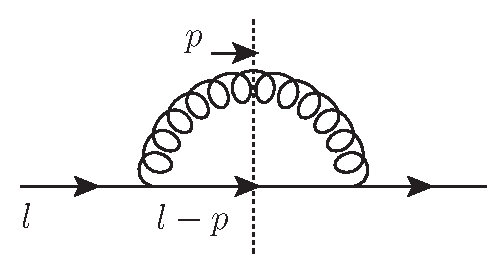
\includegraphics[width=0.3\linewidth]{selfen_gluon_cut}
  \caption{
  }
  \label{fig:selfen}
\end{figure*}

Let us focus first on the integral. The formula is
\begin{equation}
\begin{split} 
A \slashed{l} + B m &= -\frac{g^2}{(2 \pi)^2} \int d^4 p\,  \gamma_5 
(\slashed{l}-\slashed{p} +m) \gamma_5 \ \delta\bigl[p^2 - m_{\pi}^2\bigr]
\delta\bigl[(l-p)^2 - m^2\bigr]
\\
&= \frac{g^2}{(2 \pi)^2} \int d^4 p\, 
(\slashed{l}-\slashed{p} -m)  \ 
\delta\bigl[p^2 - m_{\pi}^2\bigr]
\delta\bigl[(l-p)^2 - m^2\bigr]
\\
&=  \frac{g^2}{(2 \pi)^2} (\slashed{l} -m) \int d^4 p \, 
\delta\bigl[p^2 - m_{\pi}^2\bigr]
\delta\bigl[(l-p)^2 - m^2\bigr]
-
\frac{g^2}{(2 \pi)^2} 
\int d^4 p
\ \slashed{p} \ \delta\bigl[p^2 - m_{\pi}^2\bigr]
\delta\bigl[(l-p)^2 - m^2\bigr].
\end{split}
\end{equation} 
The last term must be proportional to $\slashed{l}$. We can therefore write
\begin{equation}
\int d^4 p
\ \slashed{p} \ \delta\bigl[p^2 - m_{\pi}^2\bigr]
\delta\bigl[(l-p)^2 - m^2\bigr]
=
\slashed{l} \ F_1 
\end{equation} 
where
\begin{equation}
\begin{split} 
F_1 &= \frac{1}{l^2}\int d^4 p \  l \cdot p \ \delta\bigl[p^2 - m_{\pi}^2\bigr]
\delta\bigl[(l-p)^2 - m^2\bigr]
\\
&= \frac{1}{2}\biggl(1-\frac{m^2-m_{\pi}^2}{l^2}\biggr)
\int d^4 p \  \delta\bigl[p^2 - m_{\pi}^2\bigr]
\delta\bigl[(l-p)^2 - m^2\bigr].
\end{split} 
\end{equation} 
In summary, we obtain
\begin{equation} 
\begin{split} 
A \slashed{l} + B m &= 
\frac{g^2}{(2 \pi)^2}\biggl[ (\slashed{l} -m) - \slashed{l} \frac{1}{2}\biggl(1-\frac{m^2-m_{\pi}^2}{l^2}\biggr) \biggr] \int d^4 p \, 
\delta\bigl[p^2 - m_{\pi}^2\bigr]
\delta\bigl[(l-p)^2 - m^2\bigr]
\\
&= \frac{g^2}{(2 \pi)^2}\biggl[
\frac{1}{2}\biggl(1+\frac{m^2-m_{\pi}^2}{l^2}\biggr) \slashed{l}
-m \biggr] \int d^4 p \, 
\delta\bigl[p^2 - m_{\pi}^2\bigr]
\delta\bigl[(l-p)^2 - m^2\bigr]
\end{split} 
\end{equation} 

We can further write the explicit result for the last integral
\begin{equation} 
I_1  = 
\int d^4 p \, 
\delta\bigl[p^2 - m_{\pi}^2\bigr]
\delta\bigl[(l-p)^2 - m^2\bigr]
 =  \frac{\pi}{2 l^2} \sqrt{ \lambda(l^2,m^2,m_{\pi}^2)}
	\;\theta(l^2 -(m+m_{\pi})^2) \,
\end{equation} 
where we have introduced the so-called K\"allen function, 
$\lambda(l^2,m^2,m_{\pi}^2)=[l^2 -(m+m_{\pi})^2][l^2 -(m-m_{\pi})^2]$.

To simplify the discussion, let us take the limit $m \to 0$. We obtain
\begin{equation}
\begin{split} 
\Xi (l^2) =
\frac{1}{l^4}
 A\, l^2  \slashed{l} 
= \frac{g^2}{16 \pi\, l^6} \bigl(l^2-m_{\pi}^2\bigr)^2 
\;\theta\bigl(l^2 - m_{\pi}^2\bigr)
 \slashed{l} 
\end{split} 
\end{equation} 


\bibliographystyle{myrevtex}
\bibliography{mybiblio}

\end{document}
